\begin{figure}[H]
%\begin{center}
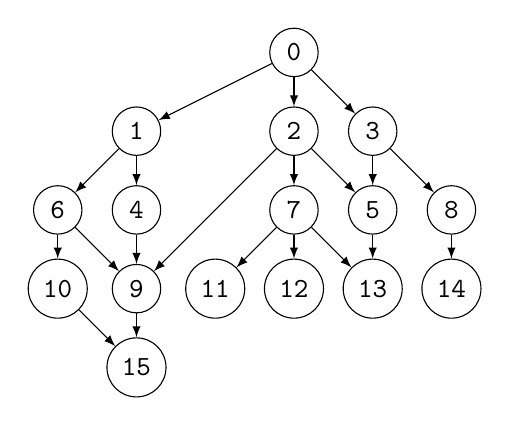
\begin{tikzpicture}[->,>=latex,auto,node distance=2.5cm,main node/.style={circle,draw,font=\ttfamily}]

  \foreach \place/\x in {
    {(3,4)/0},
    {(1,3)/1}, 
    {(3,3)/2},
    {(4,3)/3},
    {(1,2)/4}, 
    {(4,2)/5}, 
    {(0,2)/6}, 
    {(3,2)/7}, 
    {(5,2)/8},
    {(1,1)/9},
    {(0,1)/10},
    {(2,1)/11},
    {(3,1)/12},
    {(4,1)/13},
    {(5,1)/14},
    {(1,0)/15}}
  \node[main node] (\x) at \place {\x};
  
  \path[every node/.style={font=\small}]
    (0) edge (1)
    (0) edge (2)
    (0) edge (3)
    (1) edge (4)
    (1) edge (6)
    (2) edge (5)
    (2) edge (7)
    (2) edge (9)
    (3) edge (5)
    (3) edge (8)
    (4) edge (9)
    (5) edge (13)
    (6) edge (9)
    (6) edge (10)
    (7) edge (11)
    (7) edge (12)
    (7) edge (13)
    (8) edge (14)
    (9) edge (15)
    (10) edge (15);
\end{tikzpicture}
%\end{center}
\end{figure}